\chapter{Sweep line algorithms}

\index{sweep line}

Many geometric problems can be solved using
\key{sweep line} algorithms.
The idea in such algorithms is to represent
an instance of the problem as a set of events that correspond
to points in the plane.
The events are processed in increasing order
according to their x or y coordinates.

As an example, consider the following problem:
There is a company that has $n$ employees,
and we know for each employee their arrival and
leaving times on a certain day.
Our task is to calculate the maximum number of
employees that were in the office at the same time.

The problem can be solved by modeling the situation
so that each employee is assigned two events that
correspond to their arrival and leaving times.
After sorting the events, we go through them
and keep track of the number of people in the office.
For example, the table
\begin{center}
\begin{tabular}{ccc}
person & arrival time & leaving time \\
\hline
John & 10 & 15 \\
Maria & 6 & 12 \\
Peter & 14 & 16 \\
Lisa & 5 & 13 \\
\end{tabular}
\end{center}
corresponds to the following events:
\begin{center}
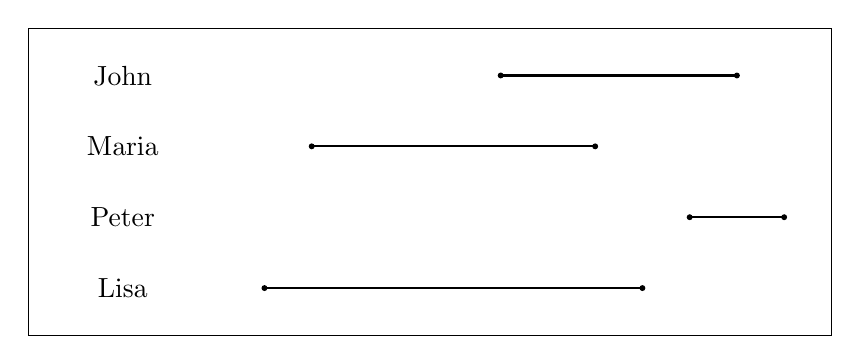
\begin{tikzpicture}[scale=0.6]
\draw (0,0) rectangle (17,-6.5);
\path[draw,thick,-] (10,-1) -- (15,-1);
\path[draw,thick,-] (6,-2.5) -- (12,-2.5);
\path[draw,thick,-] (14,-4) -- (16,-4);
\path[draw,thick,-] (5,-5.5) -- (13,-5.5);

\draw[fill] (10,-1) circle [radius=0.05];
\draw[fill] (15,-1) circle [radius=0.05];
\draw[fill] (6,-2.5) circle [radius=0.05];
\draw[fill] (12,-2.5) circle [radius=0.05];
\draw[fill] (14,-4) circle [radius=0.05];
\draw[fill] (16,-4) circle [radius=0.05];
\draw[fill] (5,-5.5) circle [radius=0.05];
\draw[fill] (13,-5.5) circle [radius=0.05];

\node at (2,-1) {John};
\node at (2,-2.5) {Maria};
\node at (2,-4) {Peter};
\node at (2,-5.5) {Lisa};
\end{tikzpicture}
\end{center}
We go through the events from left to right
and maintain a counter.
Always when a person arrives, we increase
the value of the counter by one,
and when a person leaves,
we decrease the value of the counter by one.
The answer to the problem is the maximum
value of the counter during the algorithm.

In the example, the events are processed as follows:
\begin{center}
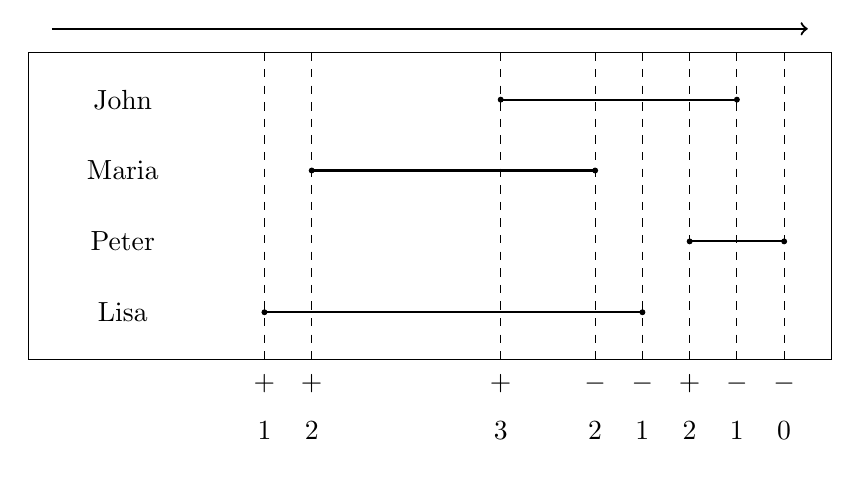
\begin{tikzpicture}[scale=0.6]
\path[draw,thick,->] (0.5,0.5) -- (16.5,0.5);
\draw (0,0) rectangle (17,-6.5);
\path[draw,thick,-] (10,-1) -- (15,-1);
\path[draw,thick,-] (6,-2.5) -- (12,-2.5);
\path[draw,thick,-] (14,-4) -- (16,-4);
\path[draw,thick,-] (5,-5.5) -- (13,-5.5);

\draw[fill] (10,-1) circle [radius=0.05];
\draw[fill] (15,-1) circle [radius=0.05];
\draw[fill] (6,-2.5) circle [radius=0.05];
\draw[fill] (12,-2.5) circle [radius=0.05];
\draw[fill] (14,-4) circle [radius=0.05];
\draw[fill] (16,-4) circle [radius=0.05];
\draw[fill] (5,-5.5) circle [radius=0.05];
\draw[fill] (13,-5.5) circle [radius=0.05];

\node at (2,-1) {John};
\node at (2,-2.5) {Maria};
\node at (2,-4) {Peter};
\node at (2,-5.5) {Lisa};

\path[draw,dashed] (10,0)--(10,-6.5);
\path[draw,dashed] (15,0)--(15,-6.5);
\path[draw,dashed] (6,0)--(6,-6.5);
\path[draw,dashed] (12,0)--(12,-6.5);
\path[draw,dashed] (14,0)--(14,-6.5);
\path[draw,dashed] (16,0)--(16,-6.5);
\path[draw,dashed] (5,0)--(5,-6.5);
\path[draw,dashed] (13,0)--(13,-6.5);

\node at (10,-7) {$+$};
\node at (15,-7) {$-$};
\node at (6,-7) {$+$};
\node at (12,-7) {$-$};
\node at (14,-7) {$+$};
\node at (16,-7) {$-$};
\node at (5,-7) {$+$};
\node at (13,-7) {$-$};

\node at (10,-8) {$3$};
\node at (15,-8) {$1$};
\node at (6,-8) {$2$};
\node at (12,-8) {$2$};
\node at (14,-8) {$2$};
\node at (16,-8) {$0$};
\node at (5,-8) {$1$};
\node at (13,-8) {$1$};
\end{tikzpicture}
\end{center}
The symbols $+$ and $-$ indicate whether the
value of the counter increases or decreases,
and the value of the counter is shown below.
The maximum value of the counter is 3
between John's arrival and Maria's leaving.

The running time of the algorithm is $O(n \log n)$,
because sorting the events takes $O(n \log n)$ time
and the rest of the algorithm takes $O(n)$ time.

\section{Intersection points}

\index{intersection point}

Given a set of $n$ line segments, each of them being either
horizontal or vertical, consider the problem of
counting the total number of intersection points.
For example, when the line segments are
\begin{center}
\begin{tikzpicture}[scale=0.5]
\path[draw,thick,-] (0,2) -- (5,2);
\path[draw,thick,-] (1,4) -- (6,4);
\path[draw,thick,-] (6,3) -- (10,3);
\path[draw,thick,-] (2,1) -- (2,6);
\path[draw,thick,-] (8,2) -- (8,5);
\end{tikzpicture}
\end{center}
there are three intersection points:
\begin{center}
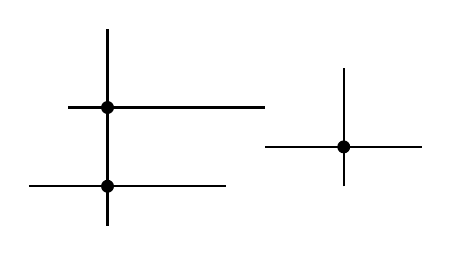
\begin{tikzpicture}[scale=0.5]
\path[draw,thick,-] (0,2) -- (5,2);
\path[draw,thick,-] (1,4) -- (6,4);
\path[draw,thick,-] (6,3) -- (10,3);
\path[draw,thick,-] (2,1) -- (2,6);
\path[draw,thick,-] (8,2) -- (8,5);

\draw[fill] (2,2) circle [radius=0.15];
\draw[fill] (2,4) circle [radius=0.15];
\draw[fill] (8,3) circle [radius=0.15];

\end{tikzpicture}
\end{center}

It is easy to solve the problem in $O(n^2)$ time,
because we can go through all possible pairs of line segments
and check if they intersect.
However, we can solve the problem more efficiently
in $O(n \log n)$ time using a sweep line algorithm
and a range query data structure.

The idea is to process the endpoints of the line
segments from left to right and 
focus on three types of events:
\begin{enumerate}[noitemsep]
\item[(1)] horizontal segment begins
\item[(2)] horizontal segment ends
\item[(3)] vertical segment
\end{enumerate}

The following events correspond to the example:
\begin{center}
\begin{tikzpicture}[scale=0.6]
\path[draw,dashed] (0,2) -- (5,2);
\path[draw,dashed] (1,4) -- (6,4);
\path[draw,dashed] (6,3) -- (10,3);
\path[draw,dashed] (2,1) -- (2,6);
\path[draw,dashed] (8,2) -- (8,5);

\node at (0,2) {$1$};
\node at (5,2) {$2$};
\node at (1,4) {$1$};
\node at (6,4) {$2$};
\node at (6,3) {$1$};
\node at (10,3) {$2$};

\node at (2,3.5) {$3$};
\node at (8,3.5) {$3$};
\end{tikzpicture}
\end{center}

We go through the events from left to right
and use a data structure that maintains a set of
y coordinates where there is an active horizontal segment.
At event 1, we add the y coordinate of the segment
to the set, and at event 2, we remove the
y coordinate from the set.

Intersection points are calculated at event 3.
When there is a vertical segment between points
$y_1$ and $y_2$, we count the number of active
horizontal segments whose y coordinate is between
$y_1$ and $y_2$, and add this number to the total
number of intersection points.

To store y coordinates of horizontal segments,
we can use a binary indexed or segment tree,
possibly with index compression.
When such structures are used, processing each event
takes $O(\log n)$ time, so the total running
time of the algorithm is $O(n \log n)$.

\section{Closest pair problem}

\index{closest pair}

Given a set of $n$ points, our next problem is
to find two points whose Euclidean distance is minimum.
For example, if the points are
\begin{center}
\begin{tikzpicture}[scale=0.7]
\draw (0,0)--(12,0)--(12,4)--(0,4)--(0,0);

\draw (1,2) circle [radius=0.1];
\draw (3,1) circle [radius=0.1];
\draw (4,3) circle [radius=0.1];
\draw (5.5,1.5) circle [radius=0.1];
\draw (6,2.5) circle [radius=0.1];
\draw (7,1) circle [radius=0.1];
\draw (9,1.5) circle [radius=0.1];
\draw (10,2) circle [radius=0.1];
\draw (1.5,3.5) circle [radius=0.1];
\draw (1.5,1) circle [radius=0.1];
\draw (2.5,3) circle [radius=0.1];
\draw (4.5,1.5) circle [radius=0.1];
\draw (5.25,0.5) circle [radius=0.1];
\draw (6.5,2) circle [radius=0.1];
\end{tikzpicture}
\end{center}
\begin{samepage}
we should find the following points:
\begin{center}
\begin{tikzpicture}[scale=0.7]
\draw (0,0)--(12,0)--(12,4)--(0,4)--(0,0);

\draw (1,2) circle [radius=0.1];
\draw (3,1) circle [radius=0.1];
\draw (4,3) circle [radius=0.1];
\draw (5.5,1.5) circle [radius=0.1];
\draw[fill] (6,2.5) circle [radius=0.1];
\draw (7,1) circle [radius=0.1];
\draw (9,1.5) circle [radius=0.1];
\draw (10,2) circle [radius=0.1];
\draw (1.5,3.5) circle [radius=0.1];
\draw (1.5,1) circle [radius=0.1];
\draw (2.5,3) circle [radius=0.1];
\draw (4.5,1.5) circle [radius=0.1];
\draw (5.25,0.5) circle [radius=0.1];
\draw[fill] (6.5,2) circle [radius=0.1];
\end{tikzpicture}
\end{center}
\end{samepage}

This is another example of a problem
that can be solved in $O(n \log n)$ time
using a sweep line algorithm\footnote{Besides this approach,
there is also an
$O(n \log n)$ time divide-and-conquer algorithm \cite{sha75}
that divides the points into two sets and recursively
solves the problem for both sets.}.
We go through the points from left to right
and maintain a value $d$: the minimum distance
between two points seen so far.
At each point, we find the nearest point to the left.
If the distance is less than $d$, it is the
new minimum distance and we update
the value of $d$.

If the current point is $(x,y)$
and there is a point to the left
within a distance of less than $d$,
the x coordinate of such a point must
be between $[x-d,x]$ and the y coordinate
must be between $[y-d,y+d]$.
Thus, it suffices to only consider points
that are located in those ranges,
which makes the algorithm efficient.

For example, in the following picture, the
region marked with dashed lines contains
the points that can be within a distance of $d$
from the active point:

\begin{center}
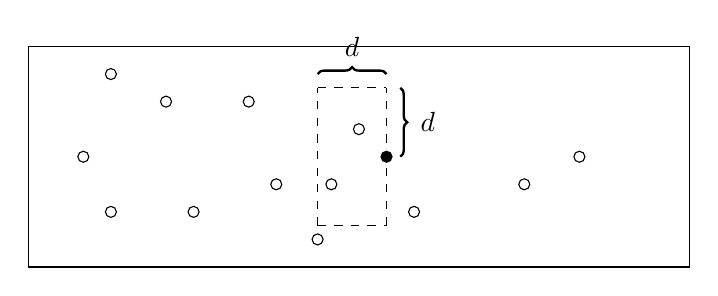
\begin{tikzpicture}[scale=0.7]
\draw (0,0)--(12,0)--(12,4)--(0,4)--(0,0);

\draw (1,2) circle [radius=0.1];
\draw (3,1) circle [radius=0.1];
\draw (4,3) circle [radius=0.1];
\draw (5.5,1.5) circle [radius=0.1];
\draw (6,2.5) circle [radius=0.1];
\draw (7,1) circle [radius=0.1];
\draw (9,1.5) circle [radius=0.1];
\draw (10,2) circle [radius=0.1];
\draw (1.5,3.5) circle [radius=0.1];
\draw (1.5,1) circle [radius=0.1];
\draw (2.5,3) circle [radius=0.1];
\draw (4.5,1.5) circle [radius=0.1];
\draw (5.25,0.5) circle [radius=0.1];
\draw[fill] (6.5,2) circle [radius=0.1];

\draw[dashed] (6.5,0.75)--(6.5,3.25);
\draw[dashed] (5.25,0.75)--(5.25,3.25);
\draw[dashed] (5.25,0.75)--(6.5,0.75);
\draw[dashed] (5.25,3.25)--(6.5,3.25);

\draw [decoration={brace}, decorate, line width=0.3mm] (5.25,3.5) -- (6.5,3.5);
\node at (5.875,4) {$d$};
\draw [decoration={brace}, decorate, line width=0.3mm] (6.75,3.25) -- (6.75,2);
\node at (7.25,2.625) {$d$};
\end{tikzpicture}
\end{center}

The efficiency of the algorithm is based on the fact
that the region always contains
only $O(1)$ points.
We can go through those points in $O(\log n)$ time
by maintaining a set of points whose x coordinate
is between $[x-d,x]$, in increasing order according
to their y coordinates.

The time complexity of the algorithm is $O(n \log n)$,
because we go through $n$ points and
find for each point the nearest point to the left
in $O(\log n)$ time.

\section{Convex hull problem}

A \key{convex hull} is the smallest convex polygon
that contains all points of a given set.
Convexity means that a line segment between
any two vertices of the polygon is completely
inside the polygon.

\begin{samepage}
For example, for the points
\begin{center}
\begin{tikzpicture}[scale=0.7]
\draw (0,0) circle [radius=0.1];
\draw (4,-1) circle [radius=0.1];
\draw (7,1) circle [radius=0.1];
\draw (6,3) circle [radius=0.1];
\draw (2,4) circle [radius=0.1];
\draw (0,2) circle [radius=0.1];

\draw (1,1) circle [radius=0.1];
\draw (2,2) circle [radius=0.1];
\draw (3,2) circle [radius=0.1];
\draw (4,0) circle [radius=0.1];
\draw (4,3) circle [radius=0.1];
\draw (5,2) circle [radius=0.1];
\draw (6,1) circle [radius=0.1];
\end{tikzpicture}
\end{center}
\end{samepage}
the convex hull is as follows:
\begin{center}
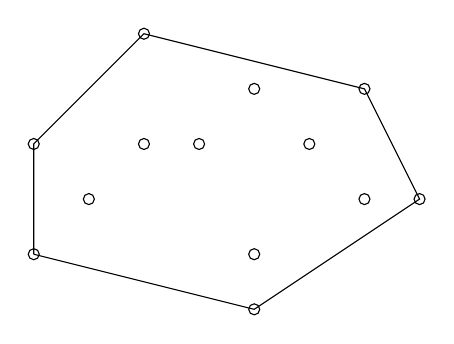
\begin{tikzpicture}[scale=0.7]
\draw (0,0)--(4,-1)--(7,1)--(6,3)--(2,4)--(0,2)--(0,0);

\draw (0,0) circle [radius=0.1];
\draw (4,-1) circle [radius=0.1];
\draw (7,1) circle [radius=0.1];
\draw (6,3) circle [radius=0.1];
\draw (2,4) circle [radius=0.1];
\draw (0,2) circle [radius=0.1];

\draw (1,1) circle [radius=0.1];
\draw (2,2) circle [radius=0.1];
\draw (3,2) circle [radius=0.1];
\draw (4,0) circle [radius=0.1];
\draw (4,3) circle [radius=0.1];
\draw (5,2) circle [radius=0.1];
\draw (6,1) circle [radius=0.1];
\end{tikzpicture}
\end{center}

\index{Andrew's algorithm}

\key{Andrew's algorithm} \cite{and79} provides
an easy way to
construct the convex hull for a set of points
in $O(n \log n)$ time.
The algorithm first locates the leftmost
and rightmost points, and then
constructs the convex hull in two parts:
first the upper hull and then the lower hull.
Both parts are similar, so we can focus on
constructing the upper hull.

First, we sort the points primarily according to
x coordinates and secondarily according to y coordinates.
After this, we go through the points and
add each point to the hull.
Always after adding a point to the hull,
we make sure that the last line segment
in the hull does not turn left.
As long as it turns left, we repeatedly remove the
second last point from the hull.

The following pictures show how
Andrew's algorithm works:
\\
\begin{tabular}{ccccccc}
\\
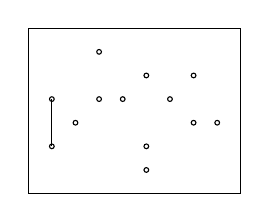
\begin{tikzpicture}[scale=0.3]
\draw (-1,-2)--(8,-2)--(8,5)--(-1,5)--(-1,-2);
\draw (0,0) circle [radius=0.1];
\draw (4,-1) circle [radius=0.1];
\draw (7,1) circle [radius=0.1];
\draw (6,3) circle [radius=0.1];
\draw (2,4) circle [radius=0.1];
\draw (0,2) circle [radius=0.1];

\draw (1,1) circle [radius=0.1];
\draw (2,2) circle [radius=0.1];
\draw (3,2) circle [radius=0.1];
\draw (4,0) circle [radius=0.1];
\draw (4,3) circle [radius=0.1];
\draw (5,2) circle [radius=0.1];
\draw (6,1) circle [radius=0.1];

\draw (0,0)--(0,2);
\end{tikzpicture}
& \hspace{0.1cm} &
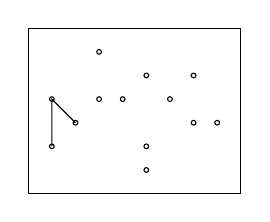
\begin{tikzpicture}[scale=0.3]
\draw (-1,-2)--(8,-2)--(8,5)--(-1,5)--(-1,-2);
\draw (0,0) circle [radius=0.1];
\draw (4,-1) circle [radius=0.1];
\draw (7,1) circle [radius=0.1];
\draw (6,3) circle [radius=0.1];
\draw (2,4) circle [radius=0.1];
\draw (0,2) circle [radius=0.1];

\draw (1,1) circle [radius=0.1];
\draw (2,2) circle [radius=0.1];
\draw (3,2) circle [radius=0.1];
\draw (4,0) circle [radius=0.1];
\draw (4,3) circle [radius=0.1];
\draw (5,2) circle [radius=0.1];
\draw (6,1) circle [radius=0.1];

\draw (0,0)--(0,2)--(1,1);
\end{tikzpicture}
& \hspace{0.1cm} &
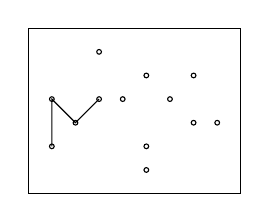
\begin{tikzpicture}[scale=0.3]
\draw (-1,-2)--(8,-2)--(8,5)--(-1,5)--(-1,-2);
\draw (0,0) circle [radius=0.1];
\draw (4,-1) circle [radius=0.1];
\draw (7,1) circle [radius=0.1];
\draw (6,3) circle [radius=0.1];
\draw (2,4) circle [radius=0.1];
\draw (0,2) circle [radius=0.1];

\draw (1,1) circle [radius=0.1];
\draw (2,2) circle [radius=0.1];
\draw (3,2) circle [radius=0.1];
\draw (4,0) circle [radius=0.1];
\draw (4,3) circle [radius=0.1];
\draw (5,2) circle [radius=0.1];
\draw (6,1) circle [radius=0.1];

\draw (0,0)--(0,2)--(1,1)--(2,2);
\end{tikzpicture}
& \hspace{0.1cm} &
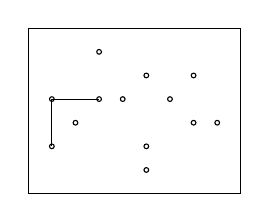
\begin{tikzpicture}[scale=0.3]
\draw (-1,-2)--(8,-2)--(8,5)--(-1,5)--(-1,-2);
\draw (0,0) circle [radius=0.1];
\draw (4,-1) circle [radius=0.1];
\draw (7,1) circle [radius=0.1];
\draw (6,3) circle [radius=0.1];
\draw (2,4) circle [radius=0.1];
\draw (0,2) circle [radius=0.1];

\draw (1,1) circle [radius=0.1];
\draw (2,2) circle [radius=0.1];
\draw (3,2) circle [radius=0.1];
\draw (4,0) circle [radius=0.1];
\draw (4,3) circle [radius=0.1];
\draw (5,2) circle [radius=0.1];
\draw (6,1) circle [radius=0.1];

\draw (0,0)--(0,2)--(2,2);
\end{tikzpicture}
\\
1 & & 2 & & 3 & & 4 \\
\end{tabular}
\\
\begin{tabular}{ccccccc}
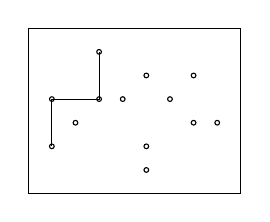
\begin{tikzpicture}[scale=0.3]
\draw (-1,-2)--(8,-2)--(8,5)--(-1,5)--(-1,-2);
\draw (0,0) circle [radius=0.1];
\draw (4,-1) circle [radius=0.1];
\draw (7,1) circle [radius=0.1];
\draw (6,3) circle [radius=0.1];
\draw (2,4) circle [radius=0.1];
\draw (0,2) circle [radius=0.1];

\draw (1,1) circle [radius=0.1];
\draw (2,2) circle [radius=0.1];
\draw (3,2) circle [radius=0.1];
\draw (4,0) circle [radius=0.1];
\draw (4,3) circle [radius=0.1];
\draw (5,2) circle [radius=0.1];
\draw (6,1) circle [radius=0.1];

\draw (0,0)--(0,2)--(2,2)--(2,4);
\end{tikzpicture}
& \hspace{0.1cm} &
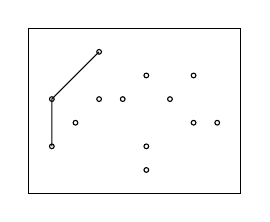
\begin{tikzpicture}[scale=0.3]
\draw (-1,-2)--(8,-2)--(8,5)--(-1,5)--(-1,-2);
\draw (0,0) circle [radius=0.1];
\draw (4,-1) circle [radius=0.1];
\draw (7,1) circle [radius=0.1];
\draw (6,3) circle [radius=0.1];
\draw (2,4) circle [radius=0.1];
\draw (0,2) circle [radius=0.1];

\draw (1,1) circle [radius=0.1];
\draw (2,2) circle [radius=0.1];
\draw (3,2) circle [radius=0.1];
\draw (4,0) circle [radius=0.1];
\draw (4,3) circle [radius=0.1];
\draw (5,2) circle [radius=0.1];
\draw (6,1) circle [radius=0.1];

\draw (0,0)--(0,2)--(2,4);
\end{tikzpicture}
& \hspace{0.1cm} &
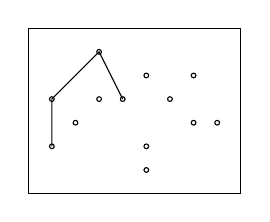
\begin{tikzpicture}[scale=0.3]
\draw (-1,-2)--(8,-2)--(8,5)--(-1,5)--(-1,-2);
\draw (0,0) circle [radius=0.1];
\draw (4,-1) circle [radius=0.1];
\draw (7,1) circle [radius=0.1];
\draw (6,3) circle [radius=0.1];
\draw (2,4) circle [radius=0.1];
\draw (0,2) circle [radius=0.1];

\draw (1,1) circle [radius=0.1];
\draw (2,2) circle [radius=0.1];
\draw (3,2) circle [radius=0.1];
\draw (4,0) circle [radius=0.1];
\draw (4,3) circle [radius=0.1];
\draw (5,2) circle [radius=0.1];
\draw (6,1) circle [radius=0.1];

\draw (0,0)--(0,2)--(2,4)--(3,2);
\end{tikzpicture}
& \hspace{0.1cm} &
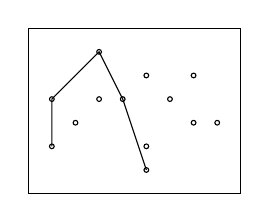
\begin{tikzpicture}[scale=0.3]
\draw (-1,-2)--(8,-2)--(8,5)--(-1,5)--(-1,-2);
\draw (0,0) circle [radius=0.1];
\draw (4,-1) circle [radius=0.1];
\draw (7,1) circle [radius=0.1];
\draw (6,3) circle [radius=0.1];
\draw (2,4) circle [radius=0.1];
\draw (0,2) circle [radius=0.1];

\draw (1,1) circle [radius=0.1];
\draw (2,2) circle [radius=0.1];
\draw (3,2) circle [radius=0.1];
\draw (4,0) circle [radius=0.1];
\draw (4,3) circle [radius=0.1];
\draw (5,2) circle [radius=0.1];
\draw (6,1) circle [radius=0.1];

\draw (0,0)--(0,2)--(2,4)--(3,2)--(4,-1);
\end{tikzpicture}
\\
5 & & 6 & & 7 & & 8 \\
\end{tabular}
\\
\begin{tabular}{ccccccc}
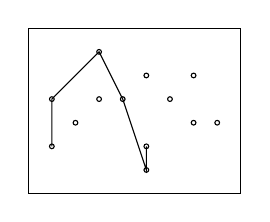
\begin{tikzpicture}[scale=0.3]
\draw (-1,-2)--(8,-2)--(8,5)--(-1,5)--(-1,-2);
\draw (0,0) circle [radius=0.1];
\draw (4,-1) circle [radius=0.1];
\draw (7,1) circle [radius=0.1];
\draw (6,3) circle [radius=0.1];
\draw (2,4) circle [radius=0.1];
\draw (0,2) circle [radius=0.1];

\draw (1,1) circle [radius=0.1];
\draw (2,2) circle [radius=0.1];
\draw (3,2) circle [radius=0.1];
\draw (4,0) circle [radius=0.1];
\draw (4,3) circle [radius=0.1];
\draw (5,2) circle [radius=0.1];
\draw (6,1) circle [radius=0.1];

\draw (0,0)--(0,2)--(2,4)--(3,2)--(4,-1)--(4,0);
\end{tikzpicture}
& \hspace{0.1cm} &
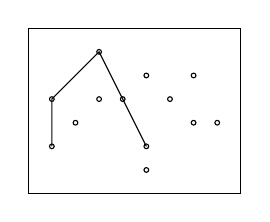
\begin{tikzpicture}[scale=0.3]
\draw (-1,-2)--(8,-2)--(8,5)--(-1,5)--(-1,-2);
\draw (0,0) circle [radius=0.1];
\draw (4,-1) circle [radius=0.1];
\draw (7,1) circle [radius=0.1];
\draw (6,3) circle [radius=0.1];
\draw (2,4) circle [radius=0.1];
\draw (0,2) circle [radius=0.1];

\draw (1,1) circle [radius=0.1];
\draw (2,2) circle [radius=0.1];
\draw (3,2) circle [radius=0.1];
\draw (4,0) circle [radius=0.1];
\draw (4,3) circle [radius=0.1];
\draw (5,2) circle [radius=0.1];
\draw (6,1) circle [radius=0.1];

\draw (0,0)--(0,2)--(2,4)--(3,2)--(4,0);
\end{tikzpicture}
& \hspace{0.1cm} &
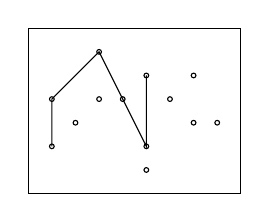
\begin{tikzpicture}[scale=0.3]
\draw (-1,-2)--(8,-2)--(8,5)--(-1,5)--(-1,-2);
\draw (0,0) circle [radius=0.1];
\draw (4,-1) circle [radius=0.1];
\draw (7,1) circle [radius=0.1];
\draw (6,3) circle [radius=0.1];
\draw (2,4) circle [radius=0.1];
\draw (0,2) circle [radius=0.1];

\draw (1,1) circle [radius=0.1];
\draw (2,2) circle [radius=0.1];
\draw (3,2) circle [radius=0.1];
\draw (4,0) circle [radius=0.1];
\draw (4,3) circle [radius=0.1];
\draw (5,2) circle [radius=0.1];
\draw (6,1) circle [radius=0.1];

\draw (0,0)--(0,2)--(2,4)--(3,2)--(4,0)--(4,3);
\end{tikzpicture}
& \hspace{0.1cm} &
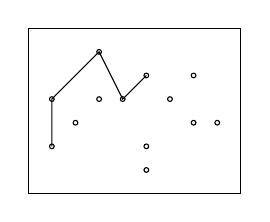
\begin{tikzpicture}[scale=0.3]
\draw (-1,-2)--(8,-2)--(8,5)--(-1,5)--(-1,-2);
\draw (0,0) circle [radius=0.1];
\draw (4,-1) circle [radius=0.1];
\draw (7,1) circle [radius=0.1];
\draw (6,3) circle [radius=0.1];
\draw (2,4) circle [radius=0.1];
\draw (0,2) circle [radius=0.1];

\draw (1,1) circle [radius=0.1];
\draw (2,2) circle [radius=0.1];
\draw (3,2) circle [radius=0.1];
\draw (4,0) circle [radius=0.1];
\draw (4,3) circle [radius=0.1];
\draw (5,2) circle [radius=0.1];
\draw (6,1) circle [radius=0.1];

\draw (0,0)--(0,2)--(2,4)--(3,2)--(4,3);
\end{tikzpicture}
\\
9 & & 10 & & 11 & & 12 \\
\end{tabular}
\\
\begin{tabular}{ccccccc}
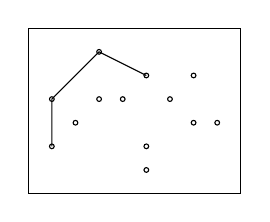
\begin{tikzpicture}[scale=0.3]
\draw (-1,-2)--(8,-2)--(8,5)--(-1,5)--(-1,-2);
\draw (0,0) circle [radius=0.1];
\draw (4,-1) circle [radius=0.1];
\draw (7,1) circle [radius=0.1];
\draw (6,3) circle [radius=0.1];
\draw (2,4) circle [radius=0.1];
\draw (0,2) circle [radius=0.1];

\draw (1,1) circle [radius=0.1];
\draw (2,2) circle [radius=0.1];
\draw (3,2) circle [radius=0.1];
\draw (4,0) circle [radius=0.1];
\draw (4,3) circle [radius=0.1];
\draw (5,2) circle [radius=0.1];
\draw (6,1) circle [radius=0.1];

\draw (0,0)--(0,2)--(2,4)--(4,3);
\end{tikzpicture}
& \hspace{0.1cm} &
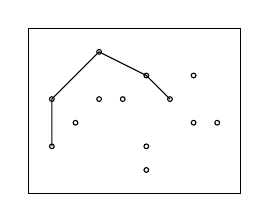
\begin{tikzpicture}[scale=0.3]
\draw (-1,-2)--(8,-2)--(8,5)--(-1,5)--(-1,-2);
\draw (0,0) circle [radius=0.1];
\draw (4,-1) circle [radius=0.1];
\draw (7,1) circle [radius=0.1];
\draw (6,3) circle [radius=0.1];
\draw (2,4) circle [radius=0.1];
\draw (0,2) circle [radius=0.1];

\draw (1,1) circle [radius=0.1];
\draw (2,2) circle [radius=0.1];
\draw (3,2) circle [radius=0.1];
\draw (4,0) circle [radius=0.1];
\draw (4,3) circle [radius=0.1];
\draw (5,2) circle [radius=0.1];
\draw (6,1) circle [radius=0.1];

\draw (0,0)--(0,2)--(2,4)--(4,3)--(5,2);
\end{tikzpicture}
& \hspace{0.1cm} &
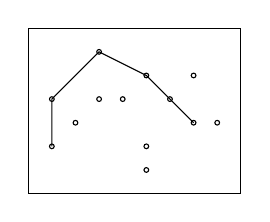
\begin{tikzpicture}[scale=0.3]
\draw (-1,-2)--(8,-2)--(8,5)--(-1,5)--(-1,-2);
\draw (0,0) circle [radius=0.1];
\draw (4,-1) circle [radius=0.1];
\draw (7,1) circle [radius=0.1];
\draw (6,3) circle [radius=0.1];
\draw (2,4) circle [radius=0.1];
\draw (0,2) circle [radius=0.1];

\draw (1,1) circle [radius=0.1];
\draw (2,2) circle [radius=0.1];
\draw (3,2) circle [radius=0.1];
\draw (4,0) circle [radius=0.1];
\draw (4,3) circle [radius=0.1];
\draw (5,2) circle [radius=0.1];
\draw (6,1) circle [radius=0.1];

\draw (0,0)--(0,2)--(2,4)--(4,3)--(5,2)--(6,1);
\end{tikzpicture}
& \hspace{0.1cm} &
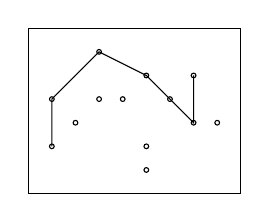
\begin{tikzpicture}[scale=0.3]
\draw (-1,-2)--(8,-2)--(8,5)--(-1,5)--(-1,-2);
\draw (0,0) circle [radius=0.1];
\draw (4,-1) circle [radius=0.1];
\draw (7,1) circle [radius=0.1];
\draw (6,3) circle [radius=0.1];
\draw (2,4) circle [radius=0.1];
\draw (0,2) circle [radius=0.1];

\draw (1,1) circle [radius=0.1];
\draw (2,2) circle [radius=0.1];
\draw (3,2) circle [radius=0.1];
\draw (4,0) circle [radius=0.1];
\draw (4,3) circle [radius=0.1];
\draw (5,2) circle [radius=0.1];
\draw (6,1) circle [radius=0.1];

\draw (0,0)--(0,2)--(2,4)--(4,3)--(5,2)--(6,1)--(6,3);
\end{tikzpicture}
\\
13 & & 14 & & 15 & & 16 \\
\end{tabular}
\\
\begin{tabular}{ccccccc}
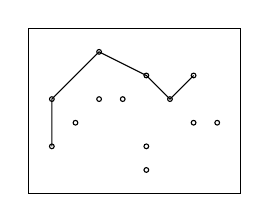
\begin{tikzpicture}[scale=0.3]
\draw (-1,-2)--(8,-2)--(8,5)--(-1,5)--(-1,-2);
\draw (0,0) circle [radius=0.1];
\draw (4,-1) circle [radius=0.1];
\draw (7,1) circle [radius=0.1];
\draw (6,3) circle [radius=0.1];
\draw (2,4) circle [radius=0.1];
\draw (0,2) circle [radius=0.1];

\draw (1,1) circle [radius=0.1];
\draw (2,2) circle [radius=0.1];
\draw (3,2) circle [radius=0.1];
\draw (4,0) circle [radius=0.1];
\draw (4,3) circle [radius=0.1];
\draw (5,2) circle [radius=0.1];
\draw (6,1) circle [radius=0.1];

\draw (0,0)--(0,2)--(2,4)--(4,3)--(5,2)--(6,3);
\end{tikzpicture}
& \hspace{0.1cm} &
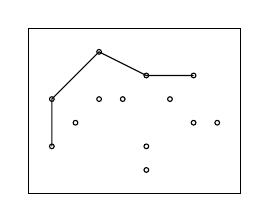
\begin{tikzpicture}[scale=0.3]
\draw (-1,-2)--(8,-2)--(8,5)--(-1,5)--(-1,-2);
\draw (0,0) circle [radius=0.1];
\draw (4,-1) circle [radius=0.1];
\draw (7,1) circle [radius=0.1];
\draw (6,3) circle [radius=0.1];
\draw (2,4) circle [radius=0.1];
\draw (0,2) circle [radius=0.1];

\draw (1,1) circle [radius=0.1];
\draw (2,2) circle [radius=0.1];
\draw (3,2) circle [radius=0.1];
\draw (4,0) circle [radius=0.1];
\draw (4,3) circle [radius=0.1];
\draw (5,2) circle [radius=0.1];
\draw (6,1) circle [radius=0.1];

\draw (0,0)--(0,2)--(2,4)--(4,3)--(6,3);
\end{tikzpicture}
& \hspace{0.1cm} &
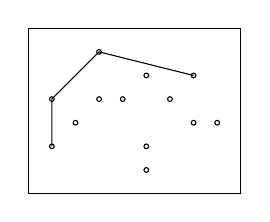
\begin{tikzpicture}[scale=0.3]
\draw (-1,-2)--(8,-2)--(8,5)--(-1,5)--(-1,-2);
\draw (0,0) circle [radius=0.1];
\draw (4,-1) circle [radius=0.1];
\draw (7,1) circle [radius=0.1];
\draw (6,3) circle [radius=0.1];
\draw (2,4) circle [radius=0.1];
\draw (0,2) circle [radius=0.1];

\draw (1,1) circle [radius=0.1];
\draw (2,2) circle [radius=0.1];
\draw (3,2) circle [radius=0.1];
\draw (4,0) circle [radius=0.1];
\draw (4,3) circle [radius=0.1];
\draw (5,2) circle [radius=0.1];
\draw (6,1) circle [radius=0.1];

\draw (0,0)--(0,2)--(2,4)--(6,3);
\end{tikzpicture}
& \hspace{0.1cm} &
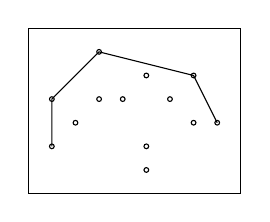
\begin{tikzpicture}[scale=0.3]
\draw (-1,-2)--(8,-2)--(8,5)--(-1,5)--(-1,-2);
\draw (0,0) circle [radius=0.1];
\draw (4,-1) circle [radius=0.1];
\draw (7,1) circle [radius=0.1];
\draw (6,3) circle [radius=0.1];
\draw (2,4) circle [radius=0.1];
\draw (0,2) circle [radius=0.1];

\draw (1,1) circle [radius=0.1];
\draw (2,2) circle [radius=0.1];
\draw (3,2) circle [radius=0.1];
\draw (4,0) circle [radius=0.1];
\draw (4,3) circle [radius=0.1];
\draw (5,2) circle [radius=0.1];
\draw (6,1) circle [radius=0.1];

\draw (0,0)--(0,2)--(2,4)--(6,3)--(7,1);
\end{tikzpicture}
\\
17 & & 18 & & 19 & & 20
\end{tabular}




